\documentclass[../main/main.tex]{subfiles}

% Put everything that shall appear in the method
% inside this document environment.
\begin{document}
	
%	\textbf{Task: describe your ideas and your realization of the task}
	
	\subsection{Designing the Questionnaire}
	
	We started out by designing a questionnaire in LaTeX \cite{lamport1994latex} and using the corporate design of our university. We clearly separated the tasks from one another and wrote the task instructions in the task headline. The body of each task consisted of task related information on the left, space for the answer in the middle and an empty coordinate system on the right. It was important to us to repeat the same structure for all tasks to increase reliability.
	
	Regarding the type of task, our choice fell on sorting tasks, because of their high objectivity (see section \ref{sec:discussion} for a discussion on task types). We decided to ask the subjects to sort five terms regarding a specific question. The first seven tasks were closed-form sorting tasks, where we already provided the first terms in a randomized order. Directly after executing each task, the subjects were asked to fill out the coordinate system with a probability density function over their performance. We used two simple, three medium and two difficult tasks. An example can be seen in figure \ref{fig:example-task}.
	
	\begin{figure}[h]
		\centering
		\captionsetup{justification=centering}
		\fbox{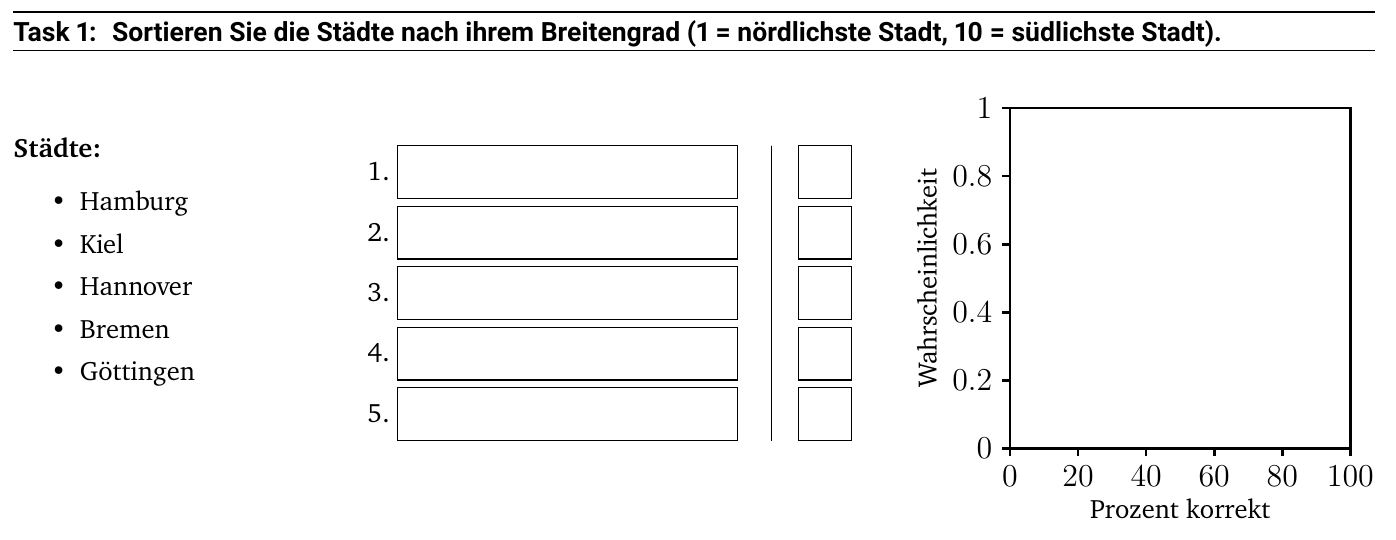
\includegraphics[width=.8\textwidth]{../assets/example-task-1.png}}
		\caption{Example closed-form sorting task.}
		\label{fig:example-task}
	\end{figure} 
	
	\noindent After the seventh task, we asked the subjects to estimate their overall performance so far. With this we hope to find some information on how well humans can average their performance over several task. 
		
	 The eighth task was an open-end sorting task, which we decided to incorporate out of curiosity. We were interested in how the self-assessment would change in comparison to closed-form sorting tasks. The task can be seen in figure \ref{fig:example-task3}.
	 
	 \begin{figure}[h]

	 	\centering
	 	\captionsetup{justification=centering}
	 	\fbox{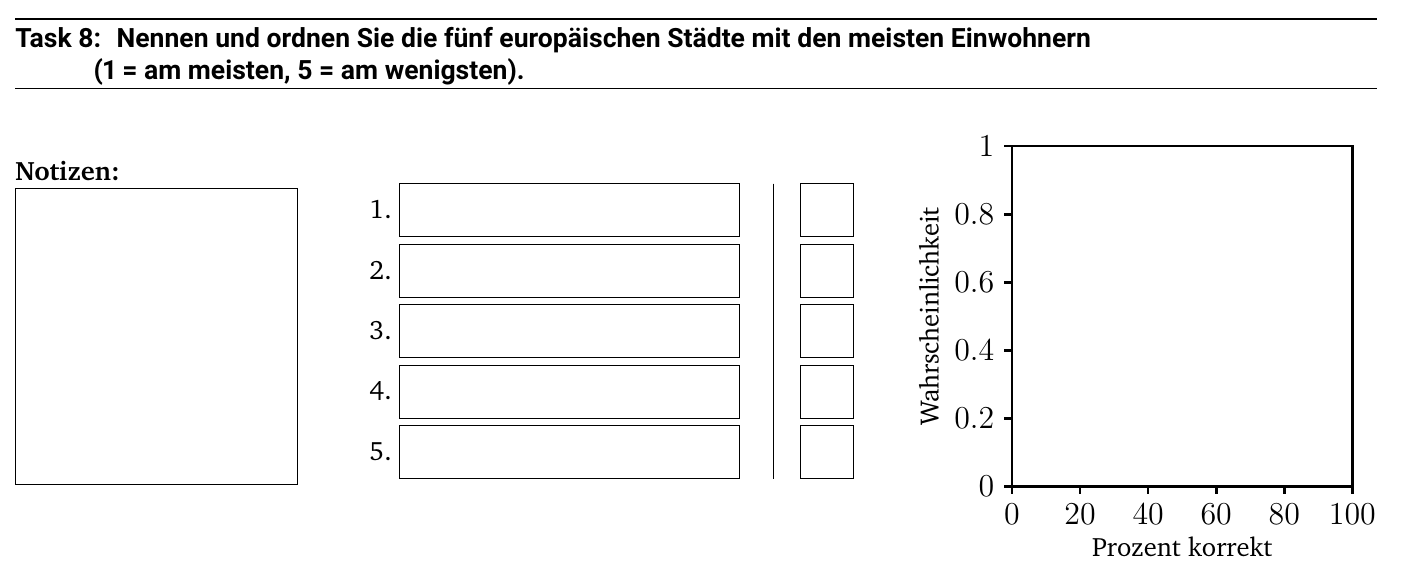
\includegraphics[width=.8\textwidth]{../assets/example-task-8.png}}
	 	\caption{Example open end sorting task.}
	 		 \label{fig:example-task3}
 	\end{figure} 
	 
	\newpage
	\subsection{Processing Pipeline}
	
	\begin{figure}[H]
	\centering
	\begin{tikzpicture}[scale=0.7, every node/.style={scale=0.7}]
		% PDF box
		\node[rectangle, draw=black, rounded corners=2mm, minimum width=3cm, minimum height=1cm, line width=1pt] 
		at (-0.6, 10.4) {\Large PDF file};
		
		% PDF arrow
		\draw[thick,arrows={-open triangle 45}]  (-7, 10.4) -- node [pos=.5, above] {scan questionnaire} (-2.4, 10.4);
		
		% Arrow PDF -> extract pdfs
		\draw[thick,arrows={-triangle 45}]  (-0.6, 9.8) -- (-0.6, 8.9) node[pos=.4, right] {\Large Extract pdfs};
		
		% --------------- Extract pdfs --------------- %
		\def\extractY{6.5}
		
		% Box
		\node[rectangle, draw=black, rounded corners=2mm, minimum width=18cm, minimum height=4.5cm, line width=1pt] 
		at (-0.8, \extractY) {};
		
		% Images
		\node[inner sep=0pt] (dist1) at (-7,\extractY)
		{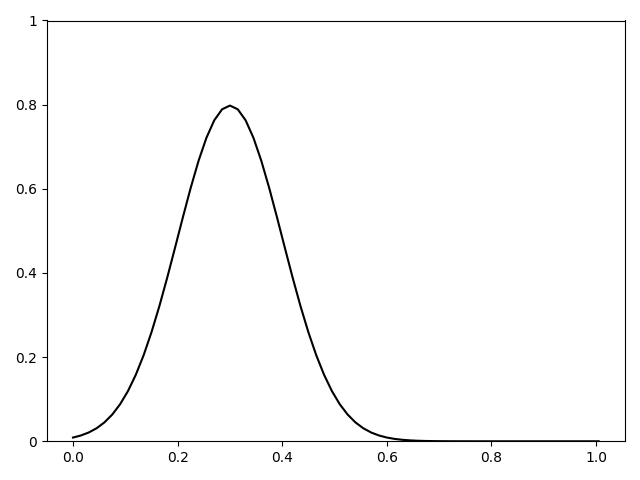
\includegraphics[width=.3\textwidth]{../assets/example_distribution_1.png}};
		\node[inner sep=0pt] (dist2) at (-1.3, \extractY)
		{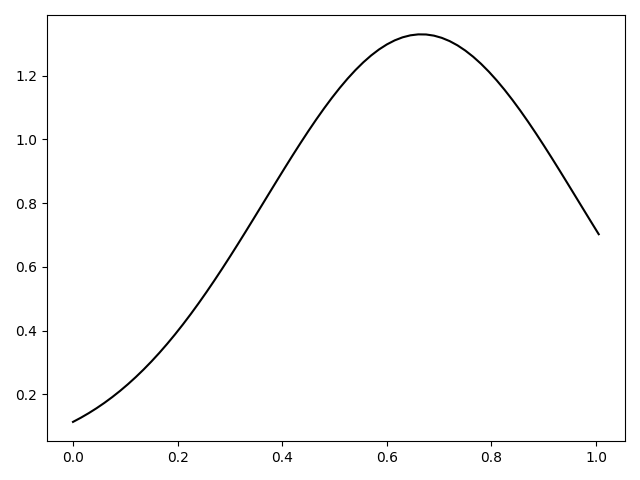
\includegraphics[width=.3\textwidth]{../assets/example_distribution_2.png}};
		\node[inner sep=0pt] (dist3) at (5,\extractY)
		{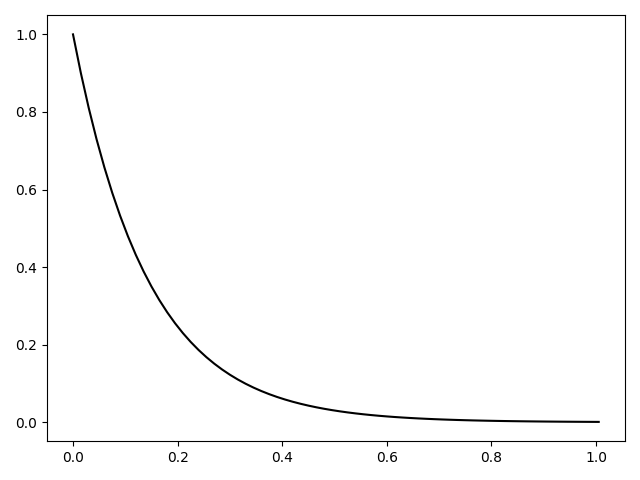
\includegraphics[width=.3\textwidth]{../assets/example_distribution_3.png}};
		
		% Points
		\node at (1.9, \extractY) {\Huge ...};
		
		% Arrow Extract -> read pdfs
		\draw[thick,arrows={-triangle 45}]  (-0.6, 4.1) -- (-0.6, 3.1) node[pos=.4, right] {\Large Read Probabilites};	

		% --------------- Read probabilities --------------- %
		
		% Box
		\node[rectangle, draw=black, rounded corners=2mm, minimum width=18cm, minimum height=4.5cm, line width=1pt] 
		at (-0.8, 0.7) {};
		
		% Images
		\node[inner sep=0pt] (dist1) at (-7,0.7)
		{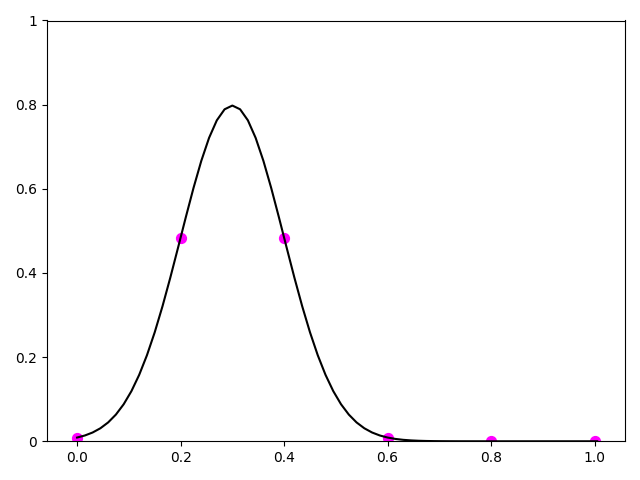
\includegraphics[width=.3\textwidth]{../assets/example_distribution_1_points.png}};
		\node[inner sep=0pt] (dist2) at (-1.3,0.7)
		{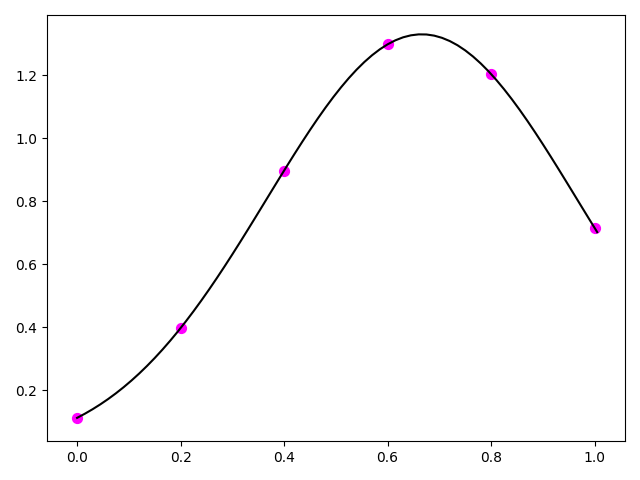
\includegraphics[width=.3\textwidth]{../assets/example_distribution_2_points.png}};
		\node[inner sep=0pt] (dist3) at (5,0.7)
		{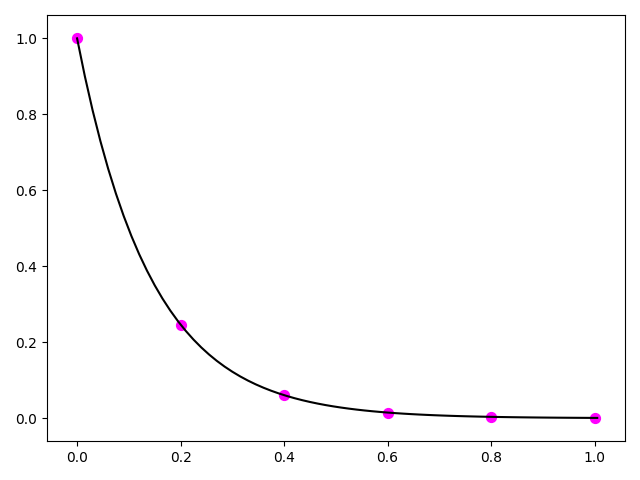
\includegraphics[width=.3\textwidth]{../assets/example_distribution_3_points.png}};
		
		% Points
		\node at (1.9, 0.7) {\Huge ...};

		% --------------- Discrete Box --------------- %
		
		% Arrow read probs -> discrete points
		\draw[thick,arrows={-triangle 45}]  (-0.6, -1.7) -- (-0.6, -2.3);
		
		% Discrete box
		\node[rectangle, draw=black, rounded corners=2mm, minimum width=5cm, minimum height=1cm, line width=1pt]  (discretebox)
		at (-0.6,-2.9) {\Large Discrete Probability Points};
		
		\draw[thick,arrows={-triangle 45}]  (-0.6, -3.5) -- (-0.6, -4.1);
		
		% --------------- Normalize --------------- %
		
		% Normalize box
		\node[rectangle, draw=black, rounded corners=2mm, minimum width=5cm, minimum height=1cm, line width=1pt]  (normalize)
		at (-0.6,-4.7) {\Large Normalization};
		
		\draw[thick,arrows={-triangle 45}]  (-0.6, -5.3) -- (-0.6, -5.9);

		% --------------- Brier score --------------- %
		% Brier score box
		\node[rectangle, double, draw=black, rounded corners=2mm, minimum width=5cm, minimum height=1cm, line width=1pt]  (brier)
		at (-0.6,-6.5) {\Large Brier Score};
		
		\draw[thick,arrows={-triangle 45}] (-0.6, -7.7) -- (-0.6, -7.1) ;
		
		% --------------- Scoring --------------- %
		
		\node[rectangle, draw=black, rounded corners=2mm, minimum width=5cm, minimum height=1cm, line width=1pt]  (score)
		at (-0.6,-8.3) {\Large Score Answers};
		
		\draw[thick,arrows={-triangle 45}]  (-0.6, -9.5) -- (-0.6, -8.9) ;
		
		% --------------- CSV --------------- %
		
		% CSV
		\node[rectangle, draw=black, rounded corners=2mm, minimum width=3cm, minimum height=1cm, line width=1pt]  (score)
		at (-0.6,-10.1) {\Large CSV};
		
		\draw[thick,arrows={-open triangle 45}]  (-7, -10.1) -- node[pos=.5, above] {enter answers} (-2.4, -10.1);
	\end{tikzpicture}
	\caption{The processing pipeline for our questionnaire. The questionnaire is scanned and saved as a PDF file on the computer. We use methods of computer vision to extract the probability density functions and read the probabilities at certain discrete points. The number of discrete points matches the possible points that a participant can achieve for a task. We normalize the probabilities (so they sum to one) and pass these probability estimations as the first parameter to a function that calculates the Brier score. The second parameter of the function consists of the participant's answers, which we write into a CSV file and score by using the L2-norm.}
	\label{fig:processing}
	\end{figure}

	After designing the questionnaire, we implemented a processing pipeline using the programming language \textit{Python} that integrates and analyzes the data that we collect by administering the questionnaire (figure \ref{fig:processing}). We started out by digitizing the image in order to apply methods of computer vision to extract the probability density functions. For convenience, we provided two ways: either scan the questionnaire as a PDF file or photograph each page of the questionnaire and upload the pages as JPEG's. In the first case, we use the python package \textit{pdf2image} \cite{pdf2images} to convert each PDF pages into single JPEG pages, which is not necessary in the second case, because the images of the questionnaire are already available in JPEG.  

	After the digitization of the questionnaire, we use methods of computer vision to detect and extract the probability density functions as single images. From these images we built a digital representation of each probability density functions and read discrete probabilities at specific locations. Afterwards, we normalized the probabilities so they sum to one. This way, the subjects do not need to care about drawing a normalized probability function and can rather concentrate on the relation between the probabilities that they assign.
	
	For a meaningful comparison, we also needed to incorporate the answers of the subjects. We did this by providing a CSV file with the answers for each subject. Our program read the CSV files and scored the answers by applying a scoring function. We then used the task scores that each person achieved for each tasks and the normalized probabilities from the probability density functions to calculate the Brier score, which we use to quantify uncertainties.
	\\\\
	The remaining segments of this section examine the individual parts of the processing pipeline in more detail.
	
	
	\subsection{Extracting Probability Density Functions}
	
	To extract probability density functions (pdfs) from a scanned PDF into an image, we used methods from computer vision to detect the probability density functions and cut out the detected regions from the JPEG. In \textit{Python}, images are stored as an array of numbers and as soon as we get the area of the probability density function as pixel indices, we can pass these pixel indices as arguments of the array and extract the desired part of the image.
	
	The hard part is to identify the probability density functions in the image. However, we designed our questionnaire in a way that reduces the detection of pdfs to the detection of a big square. If we can reliably detect the coordinate system, which the subjects use to draw their pdfs, we can extract the pdfs.
	
	To detect squares, we needed to detect vertical and horizontal lines first, which we did by applying convolutions. Next, we extracted all the contours that could be build with horizontal and vertical lines by using the \textit{Python} library \textit{OpenCV} \cite{bradski2008learning}. This will output any form of contour, including lines, triangles, rectangles and squares. Before extracting the correct contours, we needed to sort the contours from top to bottom. To the computer all pdfs look the same, so we had to make sure that we assigned the correct pdf to the correct task by sorting it. 
	
	Next, we had to find the correct squares from the contours. We did this by iterating over the contours and testing each contour regarding some constraints:
	
	\begin{enumerate}
		\item The horizontal and vertical length of the contour had to be approximately the same length. We allowed for maximal 8\% variation. One side could be up to 8\% longer than the other side. This factor was necessary, because squares on a scan are rarely perfectly axes aligned.
		\item The square of the coordinate system had a height of exactly 4.5cm. A Din A4 paper is exactly 29.7cm high. This means that each pdf makes up for about 15\% of the image height. Allowing for some deviation, the height of the contour had to be between 10 and 20\% of the height of the JPEG. 
		\item The square of the coordinate system had a width of 4.5cm. A Din A4 paper is exactly 21cm wide. This means that each pdf makes up about 21\% of the image width. Allowing for some deviation, the width of the contour had to be between 15 and 25\% of the width of the JPEG. 
		\item Last, we excluded all contours which were lying on the left half of the page.
	\end{enumerate}

	\noindent Constraint 1 makes sure that we find squares. Constraint 2 and 3 make sure we find the squares with the correct size. Constraint 4 makes sure that we do not take any squares from the left side of the page. We designed the questionnaire in a way that all pdfs are located at the right half of the page.
	
	Because we calculate the extraction of the pdfs with percentages relative to the size of a Din A4 paper, it is independent of the DPI and resolution of the scanner or photo camera, which is used to scan the questionnaire.
	
	\subsection{Extracting probabilities from probability density functions}
	
	We now have the probability density functions (pdfs) as images and can extract probabilities form it. The number of discrete probabilities that we extract from each pdf is dependent on the task scoring. In our case, we wanted to extract six discrete points, because each answer was given a score in the range of 0 to 5. 
	
	We split the x-axis of the pdf image into six equidistant numbers. The distances between these numbers differ, depending on the resolution of the camera. If we get an image with a width of 240 pixels, we get an array with the following positions: $[0, 40, 80, 120, 180, 240]$. The positions correspond to the pixels, where we read the probabilities of the pdf. 
	
	We extract the probabilities by searching the pixels along the y-axis for a given x-axis position. The first black pixel above a certain threshold is interpreted as the probability. For example, if we found a black pixel after 120 pixels and the image has a height of 240 pixels, we enter $0.5$ for the given x-axis position. We do this for every position in the array $[0, 40, 80, 120, 180, 240]$. If we do not find a black pixel, we first look at the neighboring right pixel column and then at the neighboring left pixel column. If we did not find a black pixel yet, we extend our search to the second right pixel column and then the second left pixel column. If we did not find a black pixel in this neighborhood, the subject did not draw a curve at this point and therefore we assign zero probability.
	
	After this step, we end up with an array of probabilities. For example, if the subject drew a horizontal line at the middle of the coordinate system, we end up with $[0.5, 0.5, 0.5, 0.5, 0.5, 0.5]$. However, in most cases these probabilities do not sum to one, so we normalize them. In our case the normalization of the array would yield $[0.16, 0.16, 0.16, 0.16, 0.16, 0.16]$.
	
	\subsection{Scoring the answers}
	
	To score the answers of each subject, we applied the Euclidean norm (L2-norm) to the distance between the actual position and the chosen position of the items. As an example, we assume that  the correct order of a sorting task is $[A, B, C, D, E]$ and the subject wrote $[B, D, E, A, C]$. Translated into numbers the correct ordering always translates to $[1, 2, 3, 4, 5]$ and in this case the answer of the subject translates to $[2, 4, 5, 1, 3]$. Now we take the L2-norm, which is displayed for our toy example in equation (\ref{eq:l2}). The better the placement of the answers, the lower is the L2-norm. A result of $L2 = 0$ represents a perfect fit.
	
	\begin{equation}
		\label{eq:l2}
		L2 = \sqrt{(1-2)^2 + (2-4)^2 + (3-5)^2 + (4-1)^2  + (5 - 3)^2} \approx 4.69
	\end{equation}
	
	We then calculated the worst L2-norm possible. That is the L2-norm of the difference between the actual ordering $[1, 2, 3, 4, 5]$ an the worst possible ordering $[5, 4, 3, 2, 1]$. This resulted in the worst possible L2-norm of $\text{L2-max-norm} \approx 6.32$. We then split the interval of $[0, \text{L2-max-norm}]$ into an array of a fixed amount of equidistant numbers (in our case 6). We chose six, because we assigned a score of 0 to 5 points for each task. This led to the array of $[0, 1.27, 2.53, 3.79, 5.06, 6.32]$. The discrete rating for a task was then the 'id' of the closest value of that array compared to the L2-norm of the answer. Therefore, if a subject would get a L2-norm of $L2 = 4.69$ (equation \ref{eq:l2}), the discrete score for the task would be 4 points.
	
	\subsection{Calculating the Brier Score}
	
	To calculate the accuracy of the subjects predictions, we used the Brier score \cite{murphy1973new}. It takes the mean squared differences between the actual outcome $c_i \in \{0, 1\}$ and the probability $f_i \in [0, 1]$ assigned to each outcome (equation \ref{eq:brier_score}).
	
	An outcome of $c_i = 1$ represents the occurrence of an outcome and analogous constitutes an outcome of $c_i = 0$ that an outcome did not occur. A probability of $f_i = 1$ describes a 100\% certainty that a specific outcome will occur and a probability of $f_i = 0$ describes the certainty that an outcome will not occur. A Brier score of $BS = 0$ specifies a perfect correlation between actual outcomes and predictions. A Brier score of $BS = 2$ characterizes the worst possible accuracy of predictions, that is depicting a probability of $f_i = 1$ for an outcome that did not occur and assigning all other outcomes a probability of $f_i = 0$, including the outcome that actually occurred.
	
	We now show how we applied the Brier score to our experiment. The participant could get 0 to 5 points for each task. Figure \ref{fig:example} shows an example task result.
	
	\begin{figure}[h]
		\centering
		\begin{tabular}{c|c|c|c|c|c|c|}
			& \multicolumn{6}{c|}{Possible task points} \\
			\hline
			& 0 & 1 & 2 & 3 & 4 & 5 \\
			\hline
			$c_i$ & 0 & 0 & 1 & 0 & 0 & 0 \\
			$f_i$ & 0.2 & 0.6 & 0.2 & 0 & 0 & 0\\
		\end{tabular}
		\caption{Example task result. The subjects certainty is encoded in the probabilities $f_i$ for each possible task score. The actual outcome is encoded with $c_i \in \{0, 1\}$, where 1 displays an occurring event and 0 a non-occurring event.}
		\label{fig:example}
	\end{figure}

	The actual score that the participant got for the task is encoded with $c_i = 1$ and the other possible scores that did not occur are represented by $c_i = 0$. The participant was underconfident and gave the possible task score of 0 points a probability of 0.2, the possible task score of 1 point a probability of 0.6 and the possible task score of 2 points (which actually occurred) a probability of 0.2. If we now apply the Brier score to our data, we get a Brier score of $BS \approx 0.17$, which can be retraced in equation \ref{eq:example-brier-score}.
	
	\begin{equation}
		\label{eq:example-brier-score}
		BS = (0.2 - 0)^2 + (0.6 - 0)^2 + (0.2 - 1)^2 + (0 - 0)^2 + (0 - 0)^2 \approx 0.17
	\end{equation}
	
	\noindent With the processing pipeline in place and the Brier score at hand, we could now administer the questionnaire and start plotting and evaluating the gathered data. The results can be seen in the next section.

\end{document}